In this chapter, I'm going to contextualize the state of the art of my research work. 
Besides, I'll explain the target to reach and the solution applied.\par
Nowadays lots of businesses use Big Data for analysing and providing actionable knowledge.\\
Big Data is defined as large data sets collected from different sources such as applications, social networks and websites.\\
For this, we are seeing nowadays a rapid growth of them, which causes a rise of redundancy and corrupted data.\\
The next consequence would be an accuracy reduction if models are built from them.\\
Before developing a predictive model, Feature Selection is a necessary step to reduce the number of input variables.
Data should be pre-processed with FS before training, to reduce overfitting and improve accuracy.
\newline
Nowadays, with the large volume and variety in Big Data, FS is increasingly becoming an essential preprocessing step in machine learning algorithms \cite{kamolov2021feature}.\\
It is desirable to both reduce the computational cost of modelling and, in some cases, to improve the performance of the model.\par
Several application domains have been reported in the literature in which FS helps to solve these issues, in particular for classification tasks.
The following article \cite{forman2003extensive} has reported how FS in text mining problems contribute to discarding words with only a limited occurrence using filter methods.\\
Another domain is image processing. For example, this study  \cite{muvstra2012breast} shows us how wrapper methods are used to select the best subset of extracted features to improve accuracy in breast density classification.\\
Also in bioinformatics field is used, since could help to identify the most discriminant genes in the classification of distinguishing between healthy and tumour tissues \cite{dessi2013comparative}.\\
Feature Selection is also used before a prediction process because it helps to increase performance to get rid of irrelevant or redundant variables \cite{bagherzadeh2016tutorial}.\\  
For instance, FS was also employed in the environmental field to predict and monitor air pollution \cite{ul2022improving}, which is also one of the goals of D-DUST. 
\par
D-DUST aims to predict primary pollutants from intensive farming.\\ 
To contribute to this, I performed FS on variables from different kinds of data resources used.
The physical and chemical variables chosen are the ones that, according to the scientific literature review, are most associated with the formation of primary and secondary atmospheric PM. 
Data include satellite observations (as Sentinel-5P) that can provide high spatial and temporal resolution of air pollutants variables. \\
One purpose of D-DUST is also to combine satellite-based information with ground sensor observation and air quality/atmospheric models. Indeed, satellite observations can give us useful information, especially in rural areas where ground sensors are limited thanks to their granularity.\\
Ground monitoring stations provide air quality and meteorological data, by ensuring also the validation of satellite observations.
The most commonly used by D-DUST and this work are the ones offered by ARPA stations.
Models included are the ones that provide a forecast of atmospheric and air quality such as the \gls{cams} models.
Other data processed with FS include time-invariant territorial features such as population density, land use or vegetation indexes since are correlated to the presence of pollutants.
Information more detailed regarding the data used are collected in the case study chapter \ref{chap:case}.
\par
Feature Selection not help only to make better model performance, but also to have a better comprehension of the data that are used by ML models during training.\\ 
Indeed, an aspect taken into consideration in this work is also that a \acrshort{ml} model trained with so many features would be a black box, in which a lack of interpretability could not be able to explain the decisions taken by the \gls{aii} algorithms.\\
So it's needed to care about interpretability to discard eventually confounding variables which can suggest there is a correlation when in fact there is not, even if the model's accuracy is extremely high.\\
For example, a new paper by Alex DeGrave et al. \cite{degrave2021ai} shows that a Deep Learning model trained with improper data was taking shortcuts in COVID-19 detection on radiographs due to the position of certain markers rather than on the actual radiograph.
Another common example of this is the confounding correlation between the number of shark attacks and ice cream sales. 
The following picture (Figure \ref{fig:shark}) \cite{shark-icecream} highlights how there's no direct relationship between shark attacks and ice cream sales. Instead, they're both caused by a third factor (High temperature).\newline
\begin{figure}[H]
    \centering
    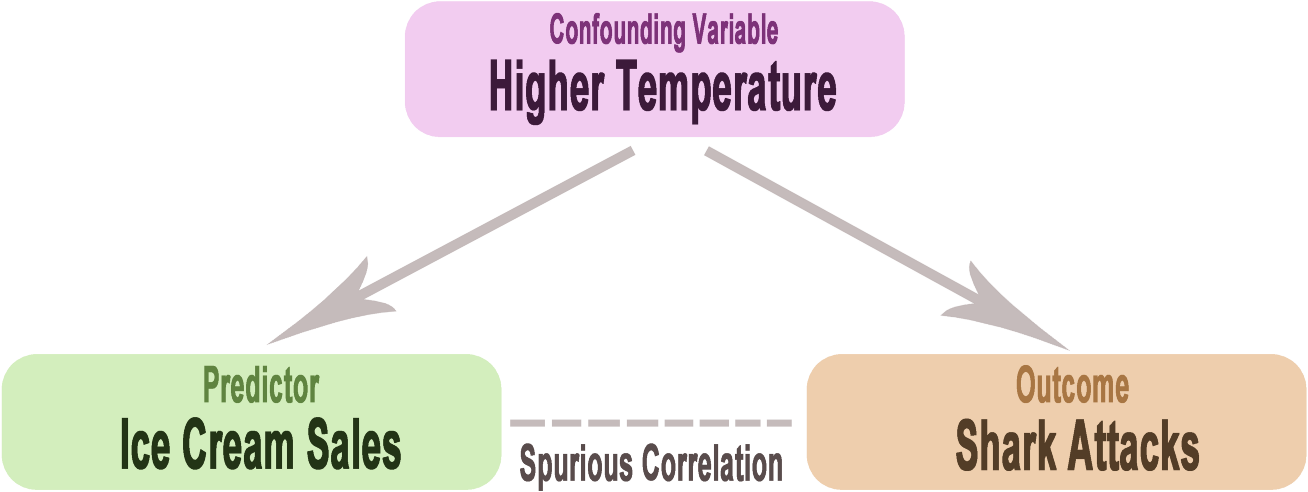
\includegraphics[scale=0.25]{images/confounding.png}
    \caption{Representation of the relationship between shark attack and ice-cream sales.}
    \label{fig:shark}
\end{figure}
Therefore, the key to increasing the interpretability of a given model is to wonder if a given factor should drive the final decision.\par
In this context, in which the black-box nature of \acrshort{ml} algorithms raises ethical and judicial concerns inducing a lack of trust \cite{9141213}, \gls{xai} aims to create a fully interpretable model.\\
Before the advent of XAI, the scientific community was focused on the predictive power of algorithms rather than the understanding behind these predictions.\\
This need for reliable high-performing models led to XAI, a field focused on the interpretation of how AI systems take decisions.
This issue of interpretability and clarity is becoming increasingly significant nowadays. \\
This is consistent with what could be seen in the figures \ref{fig:AI_XAI}.
The following figures show that publications with the words \gls{dl} and Explainable AI increased between 2010 and 2020. 
In addition, the trend of Explainable AI grew up in the last 3 years, while the curve of DL seems to have reached a saturation state.\\
\begin{figure}[H]
\centering
    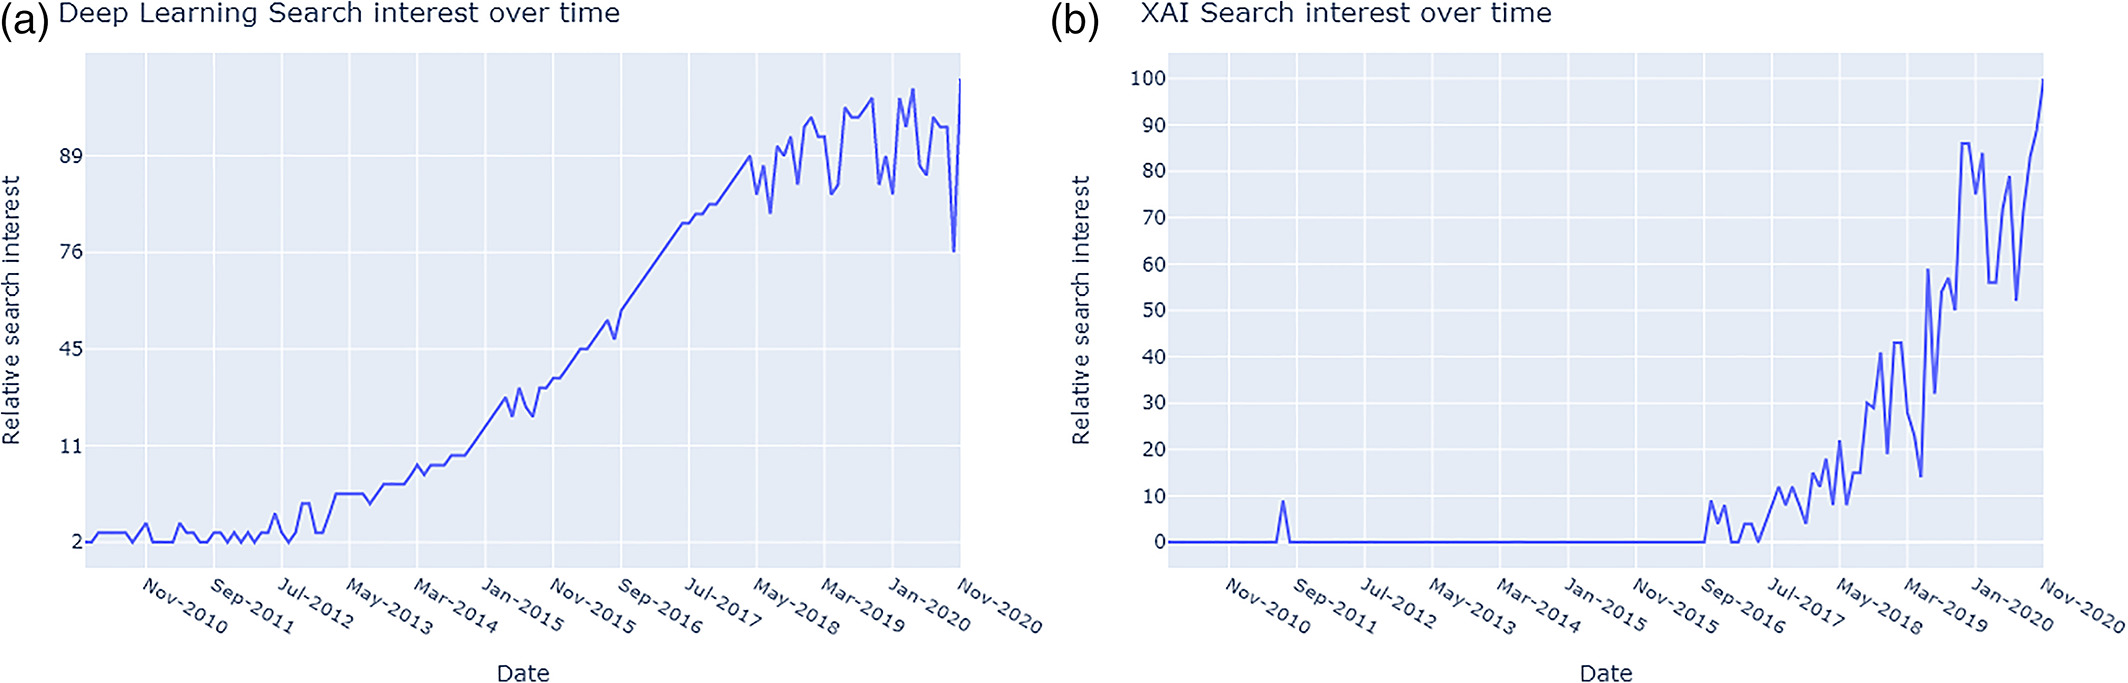
\includegraphics[scale=0.30]{images/DL-XAI.jpg}
    \caption{Plot of the interest progression of DL and XAI provided by Google Trend in the period between 2010 and 2020 \cite{angelov2021explainable}.}
    \label{fig:AI_XAI}
\end{figure}
In this work, the focus is on model interpretability instead of explainability, even if in literature there are references that describe them in the same way.\\
Interpretable Artificial Intelligence (or Interpretable Machine Learning) helps to understand how \acrshort{ml} algorithms make predictions, with the use of feature selection methods to clarify the model decision.
\par
Feature selection can provide relevant explanations by quantifying the influence of each input variable on the model's output with a score.\\
The contribution of FS will be afterwards considered during the development of ML models by D-DUST.\\
This step aims to provide a weighted score of each environmental variable considering the pollutants emitted by intensive farming activities as target variables (e.g PM2.5 and Ammonia). \\
In this work, scores will be interpreted with findings in the literature to confirm them.\\
Because there is no best feature selection technique, I performed and combined different supervised methods. \\
Then, the most weighted input variables will be used as predictors inside the D-DUST project to monitor primary pollutants from intensive farming with data science techniques, such as ML models.\\
In my work, after the reduction of the variables was made by FS, I also built 2 ML models to predict target variables related to intensive farming activities such as PM2.5 and ammonia.
\bigbreak
According to the above, my work comes in this scenario.
In the next chapter, the FS procedure will be described in detail.
\\
